\section{Instala\c{c}\~ao para Linux}
\begin{center}
{\textbf {Instala\c{c}\~{a}o do COQ no Linux }}\\
\end{center}
Para o download do COQ  no linux, ir at\'{e} o gerenciador de aplicativos e buscar onde baixar o programa.\\
\begin{figure}[!htb]
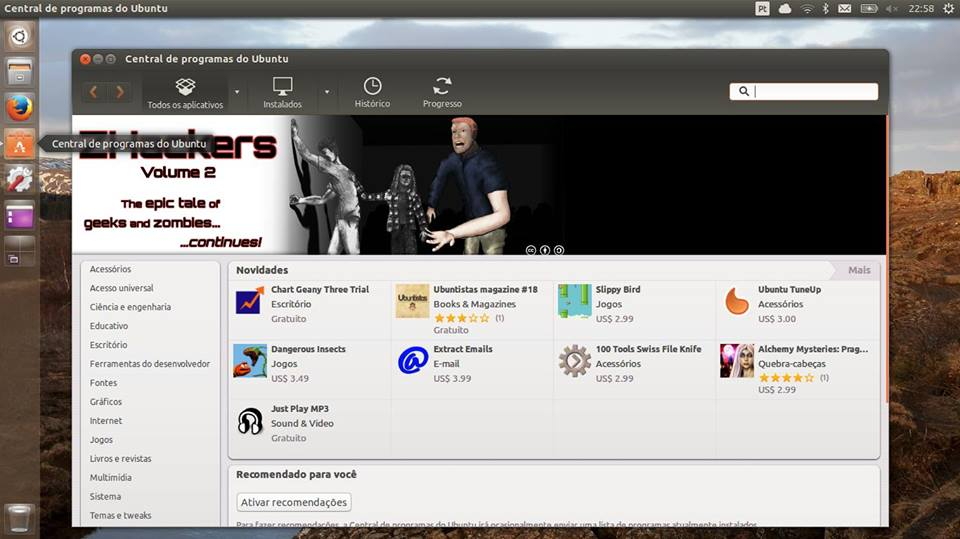
\includegraphics[scale=0.4]{imagens/linux5.jpg}
\end{figure}
Resultado da procura do coq no gerenciador:\\
\begin{figure}[!htb]
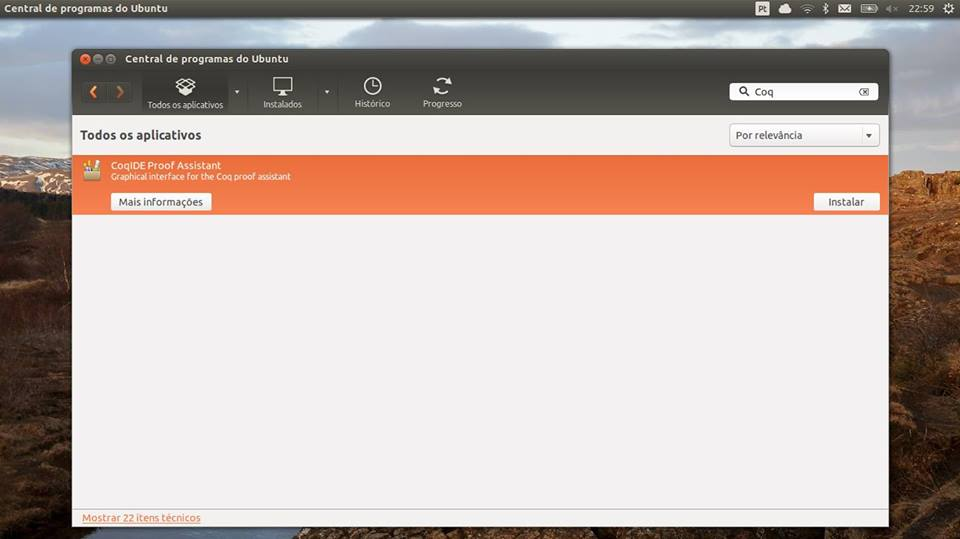
\includegraphics[scale=0.4]{imagens/linux2.jpg}
\end{figure}
Informar o usu\'{a}rio mestre do linux, o q possui os privil\'{e}gios de instala\c{c}\~{a}o de programas.\\
\begin{figure}[!htb]
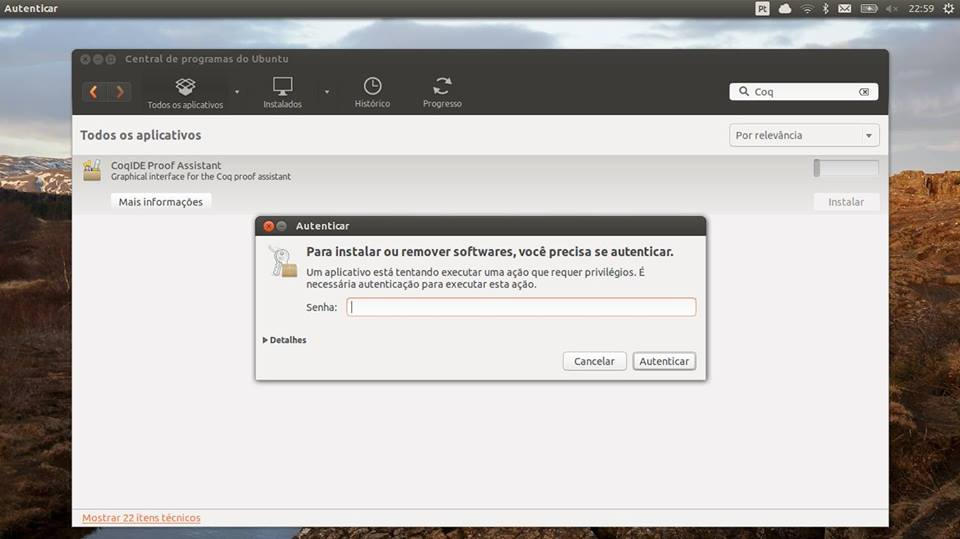
\includegraphics[scale=0.4]{imagens/linux1.jpg}
\end{figure}
Indicativo que o programa foi instalado.\\
\begin{figure}[!htb]
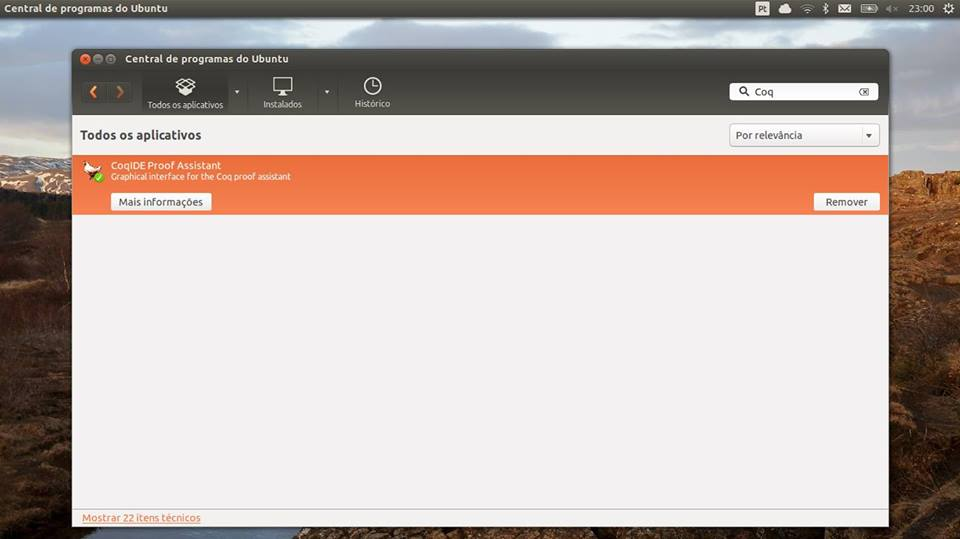
\includegraphics[scale=0.4]{imagens/linux3.jpg}
\end{figure}
Depois de instalado o \'{i}cone do Coq aparece no painel.\\
\begin{figure}[!htb]

\includegraphics[scale=0.4]{imagens/linux6.jpg}
\end{figure}
Janela do Coq aberta:\\
\begin{figure}[!htb]
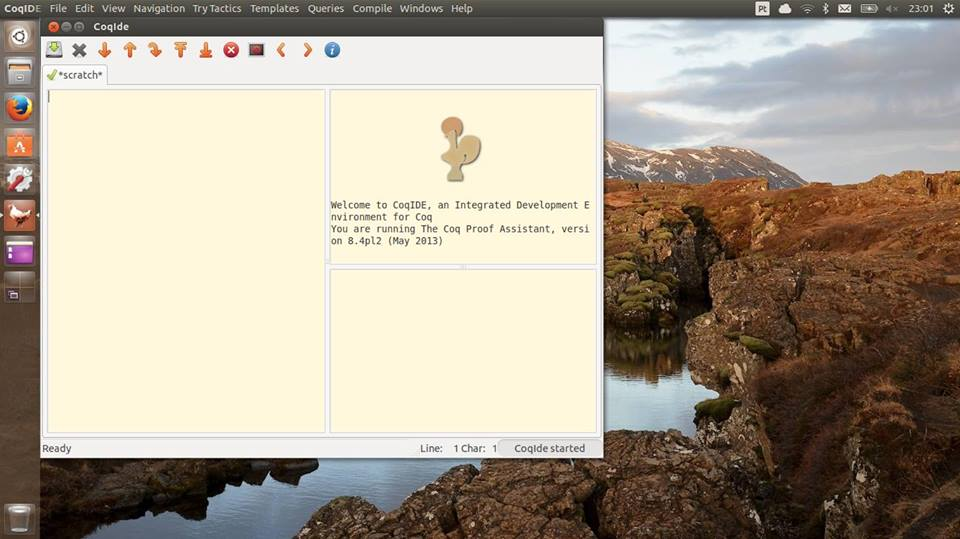
\includegraphics[scale=0.4]{imagens/linux4.jpg}
\end{figure}